\chapter{Arbeitsgrundlagen}
% ==================================================================
\setcounter{page}{1} \thispagestyle{fancy} 
% ==================================================================
Um die theoretische Quintessenz dieser Arbeit kurz zu erläutern, werden hier die \textit{\nameref{subsec:fresnelBeobachtungsart}} und die \textit{\nameref{subsec:frauenhofBeobachtungsart}} gezeigt. Dabei wird die \textit{\nameref{subsec:beugspalt}}, \textit{\nameref{subsec:beugloch}} und die \textit{\nameref{subsec:beugstrichgitter}} betrachtet.

\section{Theoretische Grundlagen}
Beugung ist die Abweichung von der geradlinigen Wellenausbreitung, mit Hilfe von Strahlen wird sie beschrieben. Wenn Wellen auf Oberflächen mit Begrenzungen, wie in dieser Arbeit z.B. der Spalt treffen, dann tritt die Beugung auf.\\[0.5cm]
Erklärt werden können diese Beugungseffekte mit Hilfe des Huygens-Fresnel’schen Prinzips. Dabei senden alle Punkte hinter einer Öffnung Sekundär-Kugelwellen aus, deren Überlagerung das neue Wellenfeld liefert. Durch diese Interferenz der Kugelwellen resultiert so mit der Fresnel'schen oder der Frauenhofer'schen Beobachtungsart ein Muster aus Licht (Maximas) und Schatten (Minimas) auf dem Schirm. Dies wird Interferenzmuster genannt\cite{Angaben2011}.\\

\subsection{Fresnel'sche Beobachtungsart}
\label{subsec:fresnelBeobachtungsart}
Um das Interferenzmuster direkt beobachten zu können wird hier ein Schirm in das Nahfeld gebracht. Mithilfe einer Linse kann dieses Muster auf einen weiter entfernteren Schirm abgebildet werden. Das Muster auf dem weiter entfernteren Schirm ist dann jedoch von der Lage der Linse (deren Brennweite) abhängig. In der Abbildung \ref{fig:Fresnel} ist die Anordnung dieser Beobachtungsart zu sehen \cite{Angaben2011}.\\[-0.5cm]
\begin{figure}[h]
\begin{center}
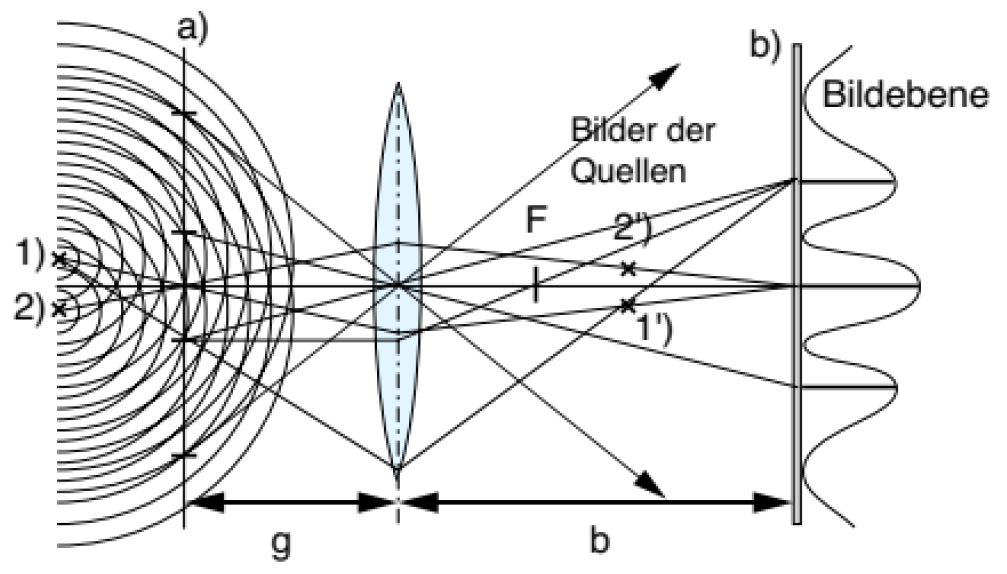
\includegraphics[scale=0.8]{Bilder/Fresnel.png} 
\end{center}
\vspace*{-0.5cm}
\caption[Anordnung der Fresnel'schen Beobachtungsart]{\textbf{Anordnung der Fresnel'schen Beobachtungsart}: Die Wellen der Quellen (1, 2) treffen auf ein Objekt (z.B Spalt) im Nahfeld (a). Die Kugelwellen interferieren dann. Über eine Linse wird das so entstehende Interferenzmuster an einen Schirm (b) \glqq projiziert\grqq\; \cite{Angaben2011}.}
\label{fig:Fresnel}
\end{figure}
\newpage

\subsection{Frauenhofer'sche Beobachtungsart}
\label{subsec:frauenhofBeobachtungsart}
Ein Schirm wird in die Brennebene einer Linse gebracht, welches das Interferenzmuster darauf abbildet. Das somit resultierende Interferenzmuster ist hier nicht von der Lage der Linse zur Quelle abhängig. In der Abbildung \ref{fig:Frauenhofer} zu erkennen.\\
\begin{figure}[h]
\begin{center}
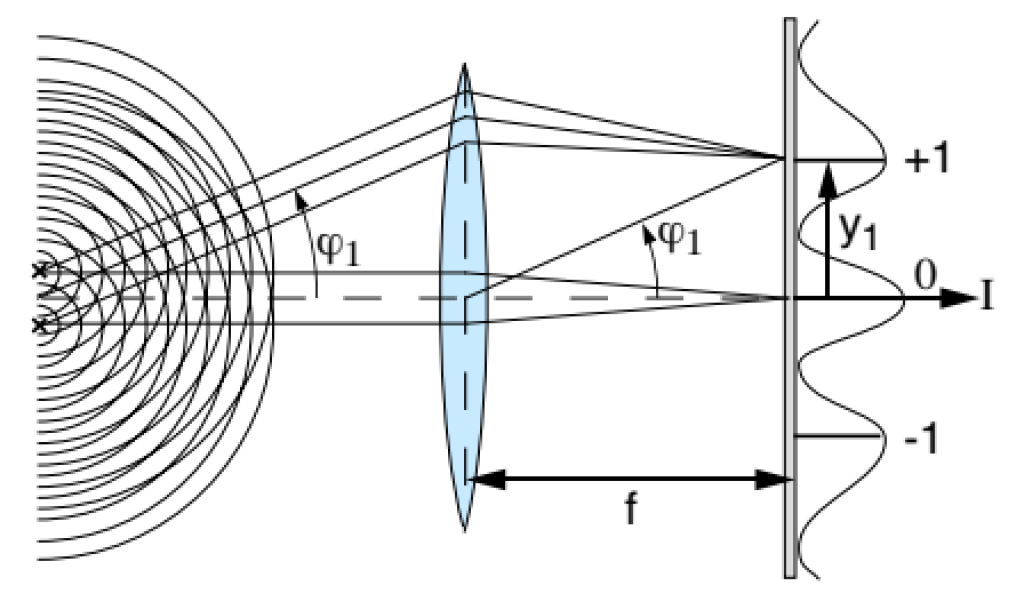
\includegraphics[scale=0.8]{Bilder/Frauenhofer.png}
\end{center}
\caption[Anordnung der Frauenhofer'schen Beobachtungsart]{\textbf{Anordnung der Frauenhofer'schen Beobachtungsart}: Das Interferenzmuster der Interferierenden Wellen wird über eine Linse im Fernfeld auf ein Schirm gegeben. Der Schirm steht in der Brennebene mit dem Abstand der Brennweite f der Linse. Das Interferenzmuster ist so unabhängig von der Linsenposition gegenüber dem Objekt \cite{Angaben2011}.}
\label{fig:Frauenhofer}
\end{figure}

Für die Beugung der Frauenhofer’sche Beobachtungsart gilt folgende Formel \ref{eq:1} \cite{Angaben2011}.\\
%FORMEL1 
\begin{equation}
a_{m}=f\cdot\tan\left( \arcsin\left[ \frac{m\cdot\lambda}{d}\right] \right) 
\label{eq:1}
\end{equation}
$a_{m}$ entspricht der Distanz des Maximums zur Mitte des Interferenzmusters. f der Brennweite. m ist repräsentativ für die Ordnungszahl. $\lambda$ steht für die Wellenlänge des He-Ne-Laserlichts (rot).\\

\subsection{Beugung am Spalt und Antispalt}
\label{subsec:beugspalt}
Beugung am Einzelspalt erzeugt im Fernfeld ein Interferenzmuster, bei welchem sich helle (Maximas) und dunkle (Minimas) Bereiche abwechseln. Die hellen Bereiche sind in der Mitte am hellsten und nach aussen gehend nimmt die Intensität ab. \cite{Angaben2011}.\\

\subsection{Beugung am Loch}
\label{subsec:beugloch}
Bei einer Lochblende wird als Interferenzmuster konzentrisch angelgte Ringe, Maxima und Minima abwechselnd auf dem Schirm beobachtet.\cite{Angaben2011}.\\[0.5cm]
Für die Auswertung bei der Beugung am Loch muss die Ordnungszahl der obigen Formel \ref{eq:1} angepasst werden, da es sich hier um Kreise handelt. Die neue Konstante, welche sich anstelle der Ordnungszahl einfügt, lässt sich gemäss folgender Formel \ref{eq:2} berechnen:
%FORMEL2
\begin{equation}
m_{i}=\frac{J_{1,i}}{\pi}
\label{eq:2}
\end{equation}

\subsubsection{Kreiskoeffizienten für Beugung am Loch}
Die ersten 9 Konstanten (m$_{i}$) werden für diese Arbeit nach der Formel \ref{eq:2} berechnet und unten dargestellt:\\[0.5cm]

\begin{tabular}[h]{ccc}
\centering
Koeffizientennummer & J$_{1,i}$ & m$_{i}$ \\ 
\hline 
1 & 3.832 & 1.220 \\  
2 & 7.016 & 2.233 \\  
3 & 10.173 & 3.238 \\ 
4 & 13.324 & 4.241 \\ 
5 & 16.471 & 5.243 \\ 
6 & 19.616 & 6.244 \\  
7 & 22.760 & 7.245 \\ 
8 & 25.904 & 8.245 \\ 
9 & 29.047 & 9.246 \\ 
\label{table:Koeff}
\end{tabular} 

\subsection{Beugung am Strichgitter}
\label{subsec:beugstrichgitter}
Bei der Beugung am Strichgitter ergibt sich ein Interferenzmuster, bei dem Lichtpunkte entlang der Horizontalen auftreten. Diese Lichtpunkte entstehen durch konstruktive Interferenz an diesen Stellen \cite{Angaben2011}.\\